\documentclass[12pt]{tcc}

% ------------- Configurações -------------
\input{config/pacotes}
\input{config/estilos}
\input{config/cores}
\input{config/comentarios}
\input{config/comandos}
\input{config/acronimos}

% ------------- Informações principais -------------
\newcommand\dtitle{Desafios de acessibilidade para idosos em aplicativos de bancos digitais}
\newcommand\dauthor{Felipe Corrêa Nogueira}
\newcommand\dadvisor{Eduardo Augusto Ferreira da Silva}

% --- Gráficos PGFPlots ---
\usepackage{pgfplots}
\pgfplotsset{compat=1.18}

% --- Necessário para usar [H] em figuras ---
\usepackage{float}

\begin{document}
\pagenumbering{gobble}
\pagenumbering{roman}

\dcover
\dcoverback

% PRECISO REVER ISSO AQUI!!!
% \includepdf{ficha.pdf}
\input{pre-textuais/dedicatoria}
\input{pre-textuais/agradecimentos}
\input{pre-textuais/epigrafe}
\input{pre-textuais/resumo}
\input{pre-textuais/abstract}

% ------------- Sumários -------------
\tableofcontents
\newpage
\listoffigures
\newpage
\listoftables

\pagenumbering{arabic}
\justifying

% --------- Capítulos -------------
\input{capitulos/1 - Introducao}
\chapter{Fundamentação Teórica}

\section{Dificuldades do Público Idoso}

Durante o processo de envelhecimento, ocorre um conjunto de alterações biológicas que desencadeiam cascatas de eventos moleculares e celulares as quais geram apoptose, radicais livres, mudanças protéicas e outros danos secundários \citep{santos2009}. Essas mudanças acabam causando um défice físico e cognitivo, entretanto, por meio de designs inteligentes e acessíveis visando a população idosa, é possível diminuir os impactos desse problema.

Um problema que atormenta a vida de muitas pessoas da terceira idade é a falta de acessibilidade no transporte público. Um estudo revela que idosos com mais limitações de mobilidade são justamente os que mais se queixam da dificuldade de acessar o transporte público e de calçadas irregulares \citep{santos2017_acessibilidade_transporte}. Como exposto anteriormente, o problema da mobilidade urbana não afeta apenas no isolamento do cidadão, mas também aumenta a dificuldade de resolver seus problemas em algum ponto de forma presencial. Diversos estudos já apontaram as dificuldades de um idoso ao tentar utilizar o transporte público, como o estudo que evidencia a falta de estrutura adequada \citep{moura2019} e o artigo que demonstra a presença de práticas etaristas nos transportes coletivos \citep{moura_freitas_2023}, mostrando que mesmo com a lei 12.587 dizendo que todos tem direito a transporte público \citep{lei_mobilidade_urbana_2012}, ainda há muito para evoluir. Entretanto, o desenvolvimento de interfaces que os usuários possam se sentir menos acuados, seria possível aumentar a qualidade de vida desse grupo populacional durante seu dia a dia, evitando os estresses urbanos que ocorrem diariamente. 

\section{Digitalização dos Bancos}

A prática de resolver seus problemas presencialmente já está sendo deixada para trás. Podemos ver em diversos aplicativos bancários como por exemplo o Bradesco, a opção de realizar diversas ações com poucos cliques.

\begin{figure}[H]
    \centering
    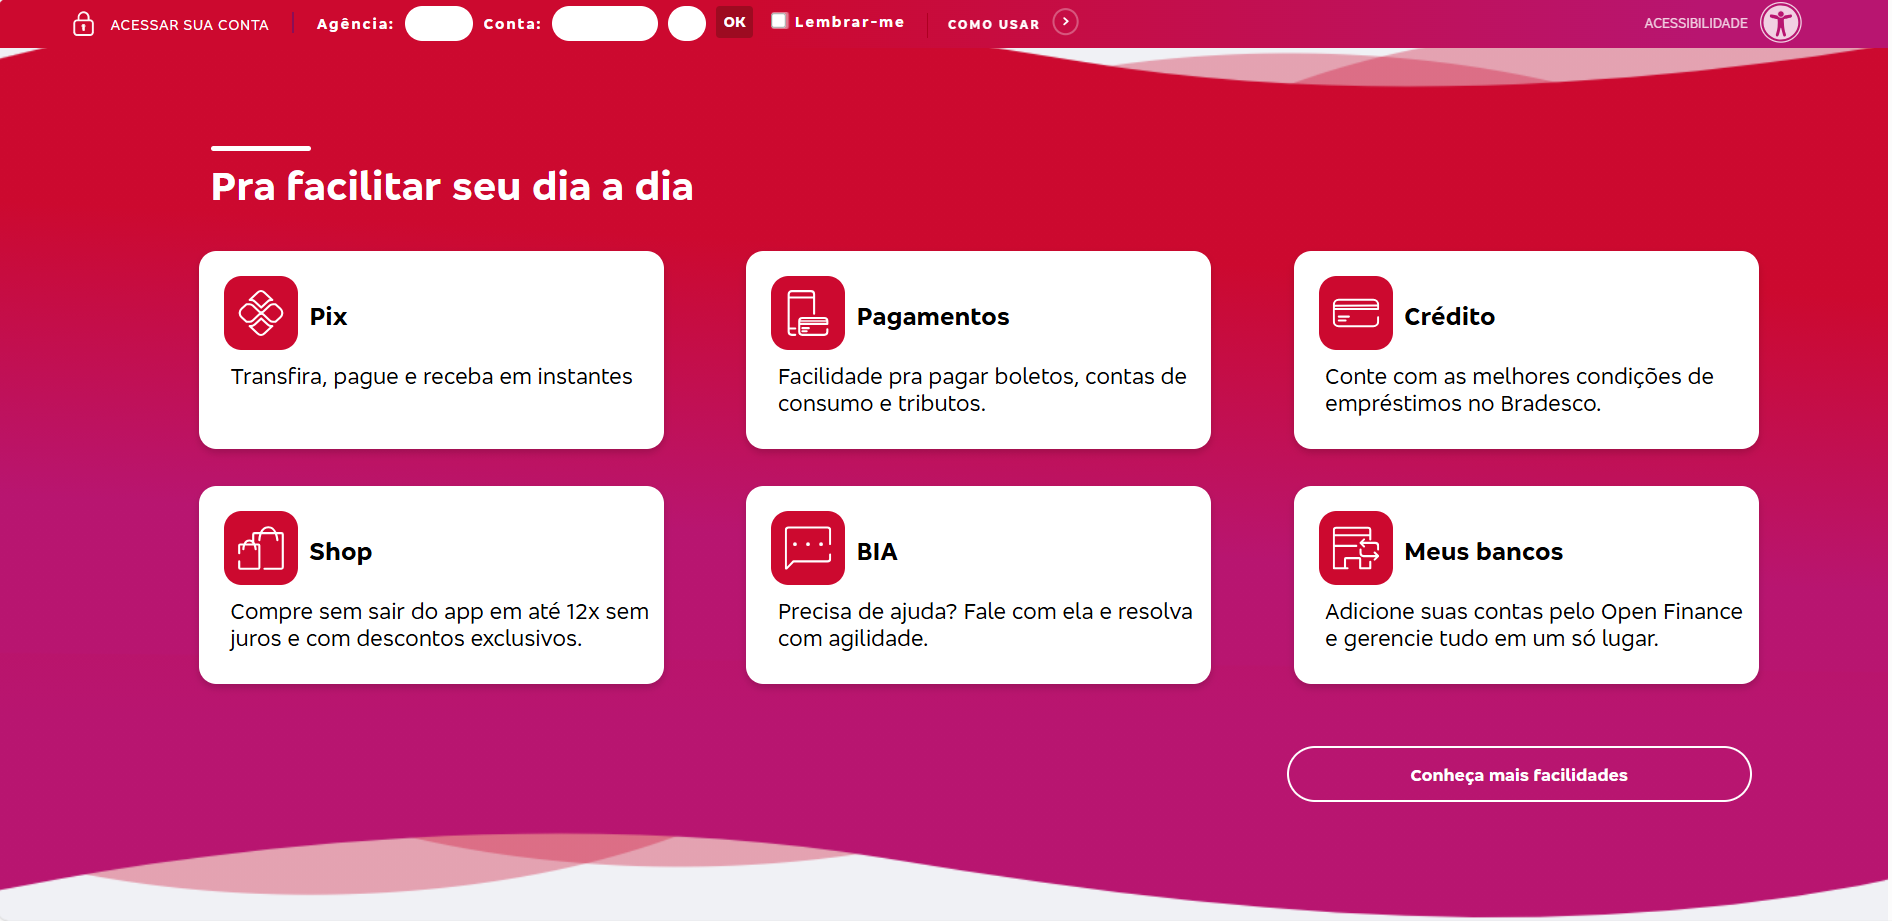
\includegraphics[width=0.9\linewidth]{imagens/Captura-de-tela-2025-11-16-210821.png}
    \caption{Funcionalidades do aplicativo Bradesco. Fonte: \citep{bradesco_app_2025}}
    \label{fig:bradesco-app}
\end{figure}

Essa tendência de digitalizar os bancos vem crescendo com os últimos anos, com a criação e popularização do NuBank, um banco 100\% digital. Chegando a ser considerada pela Forbes a sétima startup mais valiosa do mundo em 2021 \citep{forbes_nubank_2021}, foi criada com o intuito de ser uma resposta direta aos problemas que David Vélez, um dos fundadores do NuBank, e diversos consumidores brasileiros enfrentam em relação aos serviços bancários tradicionais. Rodrigo Sanchez (2021), fala sobre em seu artigo no blog Nu:

\begin{quote}
“Quando David Vélez, um dos fundadores do Nu, precisou abrir uma conta no Brasil, percebeu o quão burocrático era o sistema bancário: ter que ir até a agência, ficar preso em uma porta giratória (no Brasil estão entrando nos bancos com agentes armados) e receber maus serviços foram as experiências que “desencadearam” a mente do nosso diretor a começar a pensar numa solução, em 2012.”
\end{quote}

Todo o sucesso da NuBank reflete em como é bem vista a digitalização dos diversos processos que normalmente custariam horas e horas em filas de banco. Por conta disso, um ambiente amigável aos idosos poderia evitar de fazê-los passar por diversas dificuldades no caminho como foi exposto anteriormente, mostrando o quanto pode ser benéfico para esse público o uso de interfaces mais inclusivas para suas limitações.

\subsection*{Desafios Digitais com Idosos}

Atualmente, com os celulares de diversar marcas como Samsung e Iphone possuindo tamanhos variados entre 6 a 7 polegadas (Em centímetros, aproximadamente 15 a 17), o tamanho pequeno das opções podem causar dificuldades na navegação do aplicativo. A catarata, condição ocular que pode causar visão embaçada e distorcida é uma condição que de acordo com a OMS, causa 51\% dos casos de cegueira no mundo. Com cerca de 20 milhões de casos e 550 mil novos anualmente (citar SBO), a catarata se mostra cada vez mais presente entre os brasileiros, havendo estudos que citam essa situação, como \citep{sbbd_estendido}. 

Existe também o fator da desigualdade com relação ao tratamento de doençs oculares. Dentro da América Latina, Ásia e África, apenas 10\% das pessoas acima dos 50 anos conseguem ter suas necessidades de óculos contempladas, número que chega a 80\% em países ricos. E com relação a catarata que é um problema recorrente, sua cobertura efetiva não passa de 40\% no Brasil, dados que são expostos pelo estudo \citep{bourne2022}

\subsection*{Acessibilidade}

A acessibilidade digital vem ganhando mais atenção, visto que até existem leis exigindo a inclusão de grupos menos favorecidos. Isso não é apenas no Brasil, existindo um movimento em países no mundo a fora, como por exemplo em Portugal, onde temos o programa \citep{eusoudigital_pt}, ou nos Estados Unidos onde temos campanhas como \citep{digitalinclusionweek2025} feita pela National Digital Inclusion Alliance.

Embora muitas vezes seja vista como um tópico de qualidade do software na área de Interação Humano-Computador (IHC), e Engenharia de Software [Barbosa et al. 2021], a legislação brasileira realmente exige esse cuidado vindo dos softwares no Brasil. Entretanto, como dito por [Lago and Santos 2011], “somente a legislação não é suficiente para garantir uma prática inclusiva nas escolas”, é possível levar isso também para o contexto de acessibilidade em sistemas computacionais.

% Visando a compreender o papel da formação em Computação nesse cenário,
% [Correa et al. 2023b] avaliaram como a acessibilidade digital era abordada em Projetos
% Pedagógicos de Curso (PPCs) de graduações presenciais de Computação ofertadas por
% instituições públicas da região Centro-Oeste do país. Os resultados indicaram que os
% temas relacionados à acessibilidade digital são abordados, em geral, em disciplinas da
% área de Interação Humano-Computador (IHC). Tais disciplinas, entretanto, nem sempre
% integram o rol de componentes curriculares obrigatórios. Em um mapeamento sobre a
% perspectiva da acessibilidade como um aspecto da qualidade da IHC em diferentes cursos
% relacionados à área de Computação, foi observado que somente 46\% dos cursos tratam de acessibilidade em algum momento da formação [Camelo et al. 2023]. Tal análise evi-
% dencia a necessidade de investigar se o tema em questão é abordado, como explicitado
% nos PPCs, ou se docentes de disciplinas específicas, como IHC ou Desenvolvimento Web,
% por exemplo, extrapolam as diretrizes ementárias para tratar de acessibilidade. A pre-
% ocupação sobre incluir o tópico de acessibilidade em cursos de computação não é uma
% visão somente brasileira. Há relatos de diferentes estratégias pedagógicas para abordar o
% assunto como maneira de cobrir o assunto que muitas vezes é ausente durante a formação
% em computação [Putnam et al. 2015, Ko and Ladner 2016]

\subsection*{Design Universal}

\subsection*{Legislação e diretrizes (LBI, EMAG e WCAG)}

No Brasil e mundo afora, existem iniciativas que prezam por criar padrões para a inclusão de digital de grupos menos privilegiado. Dentro desses, no nível nacional existem a Lei Brasileira de Inclusão (LBI) e o Modelo de Acessibilidade em Governo Eletrônico (eMag), entretanto existe mundo afora o Web Content Accessibility Guidelines (WCAG).

\subsubsection{Lei Brasileira de Inclusão - LBI}

Tendo uma visão abrangente sobre quem se enquadraria como pessoa com deficiência, como mostra a citação abaixo, a LBI estabeleceu deveres concretos a serem seguidos.

\begin{quote}
"Considera-se pessoa com deficiência aquela que tem impedimento de longo prazo de natureza física, mental, intelectual ou sensorial, o qual, em interação com uma ou mais barreiras, pode obstruir sua participação plena e efetiva na sociedade em igualdade de condições com as demais pessoas."
\end{quote}

Existe também uma relação direta entre os direitos previstos na legislação brasileira e o uso de tecnologia para promover inclusão. A LBI determina que é garantido à pessoa com deficiência o acesso a produtos, recursos, estratégias, práticas, processos, métodos e serviços de tecnologia assistiva que maximizem sua autonomia, mobilidade pessoal e qualidade de vida, conforme estabelece o Art. 74 da Lei nº 13.146/2015 \citep{lei13146}.

A criação da LBI ajuda a reforçar de que a deficiência não está na pessoa, mas nas barreiras externas, como a tecnologia feita de maneira não inclusiva.

\subsubsection{Modelo de Acessibilidade em Governo Eletrônico - eMAG}

Tendo a sua última versão lançada em 2014, o eMag 3.1 trabalha como um norteador no desenvolvimento e adaptações de conteúdos digitais do governo federal. Ele serve para que os sites de instituições federais possam seguir um padrão, que também servem para ajudar outros softwares a serem mais inclusivos. Todas as informações sobre o modelo citado podem ser consultadas por qualquer usuário diretamente no site oficial do Governo Eletrônico \citep{emag2014}.

No Portal do Governo Brasileiro, são exibidas diversas imagens para exemplificar a organização padrão esperada pelo eMag. Como por exemplo as camadas de um documento web.

\begin{figure}[H]
    \centering
    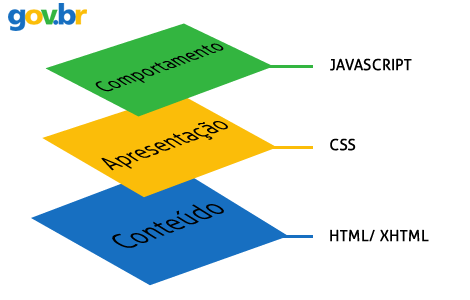
\includegraphics[width=0.9\linewidth]{imagens/camadas.png}
    \caption{Camadas de um documento web. Fonte: \citep{emag2014}}
    \label{fig:camadas-documento-web}
\end{figure}

Ou até mesmo, é possível visualizar exemplos de ordem de cabeçalhos, elementos semânticos, blocos de conteúdo, dentre outros tipos de organização.

\begin{figure}[H]
    \centering
    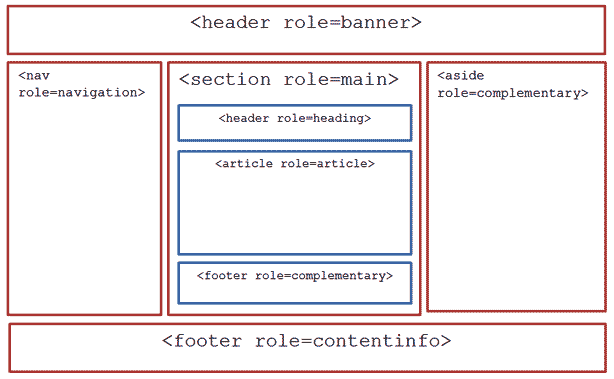
\includegraphics[width=0.9\linewidth]{imagens/estrutura_html5.png}
    \caption{Estrutura com HTML5 e ARIA. Fonte: \citep{emag2014}}
    \label{fig:estrutura-html5-aria}
\end{figure}

Entretanto o eMag não é um substituto do Web Content Accessibility Guidelines, mas sim um complemento. As regras brasileiras se tratam de uma versão especializada voltada para o governo brasileiro. Apesar disso, nenhuma boa prática dita pelo WCAG é descartável.

% Desenho Universal (DU),

Existem estudos que realizam análise de sites utilizando como base conceitos definidos por WCAG e eMAG. Entre eles, destaca-se o estudo de \citet{xavier2024}, que investiga como os princípios do governo eletrônico podem influenciar o acesso à informação pelo cidadão. Há também o estudo de \citep{batista2025}, que apesar de não tratar diretamente sobre diretrizes de acessibilidade digital, como o eMAG, ele ressalta a importância de uma infraestrutura de governo eletrônico inclusiva.

\subsubsection{Web Content Accessibility Guidelines - WCAG}

Estando na sua versão 2.2, lançada em outubro de 2023, o WCAG é uma série de diretrizes criada pelo consórcio World Wide Web (W3C) que busca manter ambientes digitais acessíveis. Ele serviu de inspiração para o eMAG, entretanto por ele ser uma adaptação focada em órgãos públicos, o WCAG acaba sendo um padrão internacional mais completo e técnico. Possuindo detalhamentos técnicos, níveis de conformidade e atualizações mais recorrentes, a W3C fornece as suas regras disponíveis em um site próprio disponível para os usuários \citep{wcag22}.

Apesar do WCAG ser consolidado e respeitado no mercado, é possível ver lacunas em seu uso, incluindo em sites brasileiros. Segundo pesquisa \citep{mwpt2022}, menos de 1\% dos sites brasileiros conseguem passar em todos os testes de acessibilidades, feitos levando as regras da W3C como parâmetro. Essa situação ocorre por conta de diversos motivos, dentre eles podem ser levados em conta a falta de capacitação, ausência de diretrizes organizacionais estruturadas e percepções equivocadas sobre o impacto no tempo e custo de desenvolvimento. Existem estudos que retratam os desafios na adoção de práticas determinadas pelo WCAG, como \citep{loiola2025} ou \citep{anaSofia2025}, que apesar de não relacionarem com o público idoso, citam o impacto e importância das regras de acessibilidade.

\subsection*{Tecnologias utilizadas}

O desenvolvimento do protótipo, pensado em uma experiência mais prática e acessível ao usuário idoso, foi feito através de ferramentas e conceitos que permitem a criação e planejamento de designs. Entre essas ferramentas destaca-se o Figma, uma plataforma colaborativa que possibilita a criação e prototipagem de interfaces digitais de forma integrada. Além disso, foram aplicados conceitos de Experiência do Usuário (UX) e Interface do Usuário (UI), garantindo que o design seguisse padrões de usabilidade e acessibilidade voltados às necessidades específicas desse público.

\subsection*{Figma}
 
Para a criação das telas, foi escolhido o Figma. Esta ferramenta funciona como uma forma de desenvolver designs colaborativos, servindo para criar interfaces e protótipos de produtos digitais. Sua popularização ocorreu por conta do número de funcionalidades que facilitam o trabalho de desenvolvedores, designers e outros profissionais que trabalham com a criação de produtos digitais \citep{figma2024}.

O Figma serve para auxiliar profissionais de Design de Produto, Design UI/UX e desenvolvedores de software. Sendo usado principalmente na criação de interfaces digitais, a plataforma ajuda com o desenvolvimento dos protótipos de aplicativo móveis, web, dentre outros \citep{figma2023}.

Com diversas funções, existem algumas que valem a pena serem citadas, pois conseguem resumir bem a experiência de desenvolvimento na ferramenta. É permitida a criação de componentes replicáveis ao longo do projeto. Relevante dizer que, todas as modificações podem ser vistas em tempom real por outros membros da equipe, permitindo a criação de protótipos interativos, com testes de usabilidade entre os membros da equipe.

\begin{figure}[H]
    \centering
    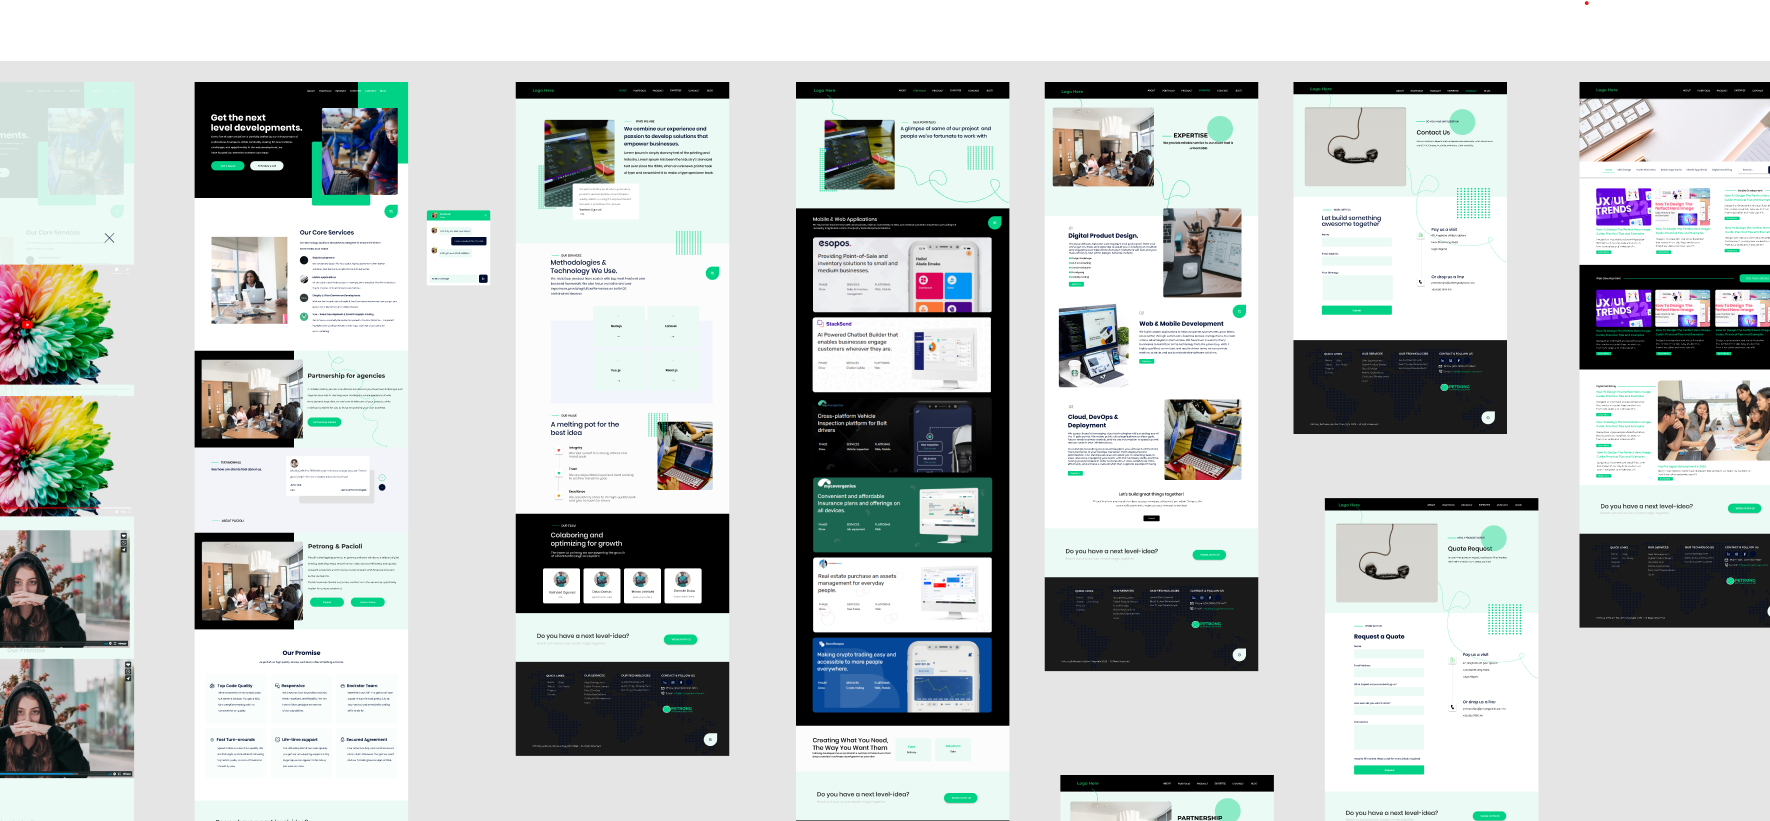
\includegraphics[width=0.9\linewidth]{imagens/Captura-de-tela-2025-12-03-205349.png}
    \caption{Imagem retirada de um projeto publicado na Comunidade do Figma. Fonte: \citep{figma_comunidade_website_project}}
    \label{fig:figma-comunidade-website-project}
\end{figure}

Além de todas as opções que o figma pode oferecer, ele ainda conta com uma comunidade engajada. Podendo oferecer tanto protótipos para serem reutilizados, quanto dicas para iniciantes.

\subsection{Conceitos utilizados}

\subsection*{Experiência do Usuário - UX}

O UX Design concentra-se na experiência do usuário dentro do aplicativo como um todo. Para garantir que o produto final seja funcional, eficiente e atenda às necessidades do usuário. É relacionado com pesquisas com público, criação de fluxos e protótipos, além de testes de uso. Os conceitos de UX buscam entender comportamentos e dificuldades que o usuário possa passar, para assim criar soluções adequadas e que melhorem a experiência.

\subsection*{Interface do Usuário - UI}

O UI Design concentra-se na parte visual e interativa do produto. Ele é responsável por projetar a aparência do que está sendo desenvolvido, incluindo ícones, botões, cores e outros elementos visuais. O plano do UI é criar um design que seja atraente, intuitivo e funcional para o usuário. Tudo para garantir que todos consigam interagir facilmente com o produto.

\label{sec:fundamentacao}

% \section{Inclusão Digital e o Público Idoso}
% \subsection{Envelhecimento e desafios tecnológicos}
% \subsection{Conceito de inclusão digital}
% \subsection{Barreiras de acesso e exclusão digital}

% \section{Acessibilidade e Design Universal}
% \subsection{Princípios de Design Universal}
% \subsection{Legislação e diretrizes (LBI e WCAG)}

% \section{Design de Interfaces Móveis}
% \subsection{Experiência do Usuário (UX)}
% \subsection{Interface do Usuário (UI)}
% \subsection{Usabilidade em dispositivos móveis}

% \section{Ferramentas e Tecnologias}
% \subsection{Figma e prototipagem colaborativa}
% \subsection{Aplicação prática dos conceitos de UX/UI}

%https://www.scielo.br/j/rbgg/a/kpmsVnswSGGRkPxYt9mKpvd/?lang=pt
\chapter{Revisão da Literatura / Trabalhos Relacionados}
Este capítulo busca expor e discutir sobre trabalhos similares ao desse TCC. Utilizando ferramentas como Google Scholar e sdc biblioteca, encontrei autores que falam sobre acessibilidade tanto de idosos quanto de outros grupos.

Explorar trabalhos que analisam o problema de acessibilidade digital com outros grupos fragéis em nossa sociedade ajuda a abranger o problema e vê-lo com outros olhos. Ver uma solução em uma situação semelhante pode ajudar na resolução a falta ambientes onlines adequados para idosos.
\label{sec:revisao}
\input{capitulos/4 - Proposta}
\input{capitulos/5 - conclusao}

\newcommand{\Extrachap}[1]{\chapter*{#1}\markboth{#1}{#1}%
\addcontentsline{toc}{chapter}{#1}}

\Extrachap{Referências}

\renewcommand{\bibsection}{}
\renewcommand{\bibname}{}

\bibliography{references}
\bibliographystyle{plainnat}

\label{bibfinalpage}

\end{document}
